\chapter{Methodology}
\label{chap:methodology}

The content of this chapter gives an answer to which steps that have to be taken to 
be able to answer the research questions.
The first section explains how electromagnetic radiation is calculated for each source
and how to convert these values to specific absorption rates. 
The second section gives a detailed overview of how a microstrip patch antenna can be 
designed and how its radiation pattern is achieved.
The third section discusses how the network can be optimized towards either electromagnetic 
exposure or power consumption.
The final section explains how these algorithms are implemented and how to further improve performance.

\section{Electromagnetic Exposure}
\subsection{Calculation of the Total Specific Absorption Rate} % (fold)
\label{sub:Calculationexposure}

The total whole body \gls{SAR} ($SAR^{wb,total}_{10g}$) (expressed in $W/kg$) of a user can be calculated by a simple sum of individual SAR values from the different sources.
Formula \ref{eq:overallSARwb} was originally described in \cite{J17_kuehn2019modelling}.
This formula assumes that the users are holding their device next to their ear and therefore 
investigates localized \gls{SAR} for head and torso area.
However for this case, this would result into incorrect conclusions since 
the position of the device relative to the user is unknown.
The position of the phone can be next to the head but also in front of the user.
The induced electromagnetic radiation will therefore be expressed in function of the entire body.


\begin{equation} 
SAR^{wb,total}_{10g} = SAR^{wb,myUE}_{10g} +  SAR^{wb,myUABS}_{10g} + SAR^{wb,otherUE}_{10g} + SAR^{wb,otherUABSs}_{10g}
\label{eq:overallSARwb}
\end{equation}

The first parameter, $SAR^{wb,myUE}_{10g}$, indicates the absorbed electromagnetic radiation by the whole body originating from the user's own device. Despite that the 
\gls{UL} radiation is destined for the serving \gls{UABS}, a portion of that radiation is directly absorbed by its user, due to the omnidirectional nature of the mobile's antenna.
The second parameter, $SAR^{wb,myUABS}_{10g}$, represents the \gls{DL} radiation caused by the \gls{UABS} that is serving the user.
As the third parameter, we have the $SAR^{wb,otherUE}_{10g}$ which is radiation caused by other people's devices. The radiation of these devices is once again 
destined for a specific \gls{UABS} but again, a portion of that \gls{UL} radiation will also be absorbed by our user.
Finally, $SAR^{wb,otherUABSs}_{10g}$ represents the \gls{DL} radiation by the other \gls{UABS}s to which our user is exposed to sbut not served by.
An illustration is given in figure \ref{fig:networkIllustration}.
We can only speak in terms of \gls{SAR}
  when the electromagnetic radiation is absorbed by the user. This last step is however not shown in the illustration.

The electromagnetic exposure to which people are exposed can be categorized in two groups. One of them is near-field radiation which is caused 
by the user's own device which is indicated with the green arrow in figure \ref{fig:networkIllustration} and will be discussed in \ref{sub:Uplinkexposure}.
The other arrows are a form of far-field radiation and will be explained in section \ref{sub:Calculatingdownlinkexpsure}. 
Examples of these types of radiators are \gls{UE} which belong to other people and \gls{UABS}s. 

\begin{figure}[h!]
\centering
  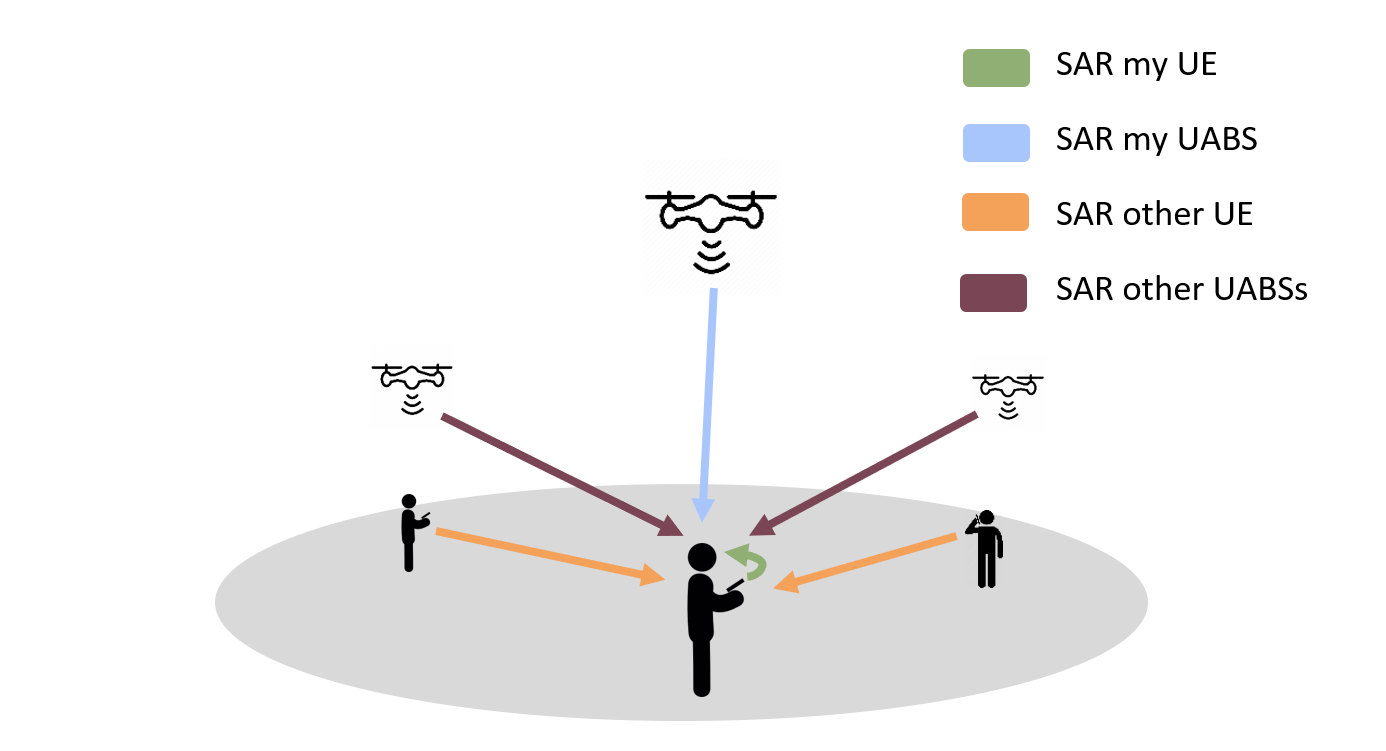
\includegraphics[width=\textwidth/3*2]{../images/networkIllustrationSARSources.png}
  \caption{Illustration of the radiation affecting the average user (here shown in the center) by different types of sources. }
  \label{fig:networkIllustration}
\end{figure}



\subsection{Electromagnetic Exposure Caused by Far-Field Radiation} % (fold)
\label{sub:Calculatingdownlinkexpsure}


\subsubsection{Electromagnetic Radiation from a Single Source}
\label{sec:calculatingexposure}

To determine the total exposure of a single human being or even of the entire network, the electric-field $\vec{E}$ from a single radiator $i$ should be calculated.
The formula to determine this electromagnetic value $E$ (expressed in V/m) for a specific location $u$ is given in equation \ref{eq:singleexposure}.

\begin{equation}
E_i(u) [V/m] = 10^{\frac{RRP(u)[dBm] - 43.15 + 20\cdot\log(f [MHz])- PL(u) [dB]}{20}}
\label{eq:singleexposure}
\end{equation}

\paragraph{Real radiation power and EIRP.}
In formula \ref{eq:singleexposure}, as it was described in \cite{J6_originalExposureFormula, J1}, 
\gls{RRP} was defined as \gls{EIRP}. \gls{EIRP} is the radiation generated by an \gls{isotropicradiator} which is
a theoretical source of electromagnetic waves that radiate with the same intensity in all directions. 
The formula to find this \gls{EIRP} value (in dBm) is described in \ref{eq:eirp}
where $P_{tx}$ stands for the input power of the antenna, $G_t$ for the gain of the transmitter and $L_t$ being its feeder loss.
\begin{equation}
EIRP [dBm] = P_{tx} [dBm] + G_t [dBi]- L_t [dB]
\label{eq:eirp}
\end{equation}
This formula, which is constructed out of different gains and losses, misses a factor when accounting for real life radiation patterns.
Formula \ref{eq:singleexposure} solves this by using \gls{RRP} instead of \gls{EIRP} and can be defined as follows:
\begin{equation}
RRP(u) [dBm] = EIRP [dBm] - attenuation(u) [dB]
\label{eq:rrp}
\end{equation}
The attenuation for a user $u$ is given based on the angle between the main beam and the user. More details on how this can be implemented are described where the radiation patters of antennae are explained.
When assuming that $attenuation(u)$ returns positive values, the attenuation can simply be subtracted from the EIRP-value.

\paragraph{frequency}
The used frequency in the formula above is denoted as $f$ and is expressed in MHz. Since LTE is used, this value will be 2600 MHz.

\paragraph{path loss}
\label{subsec:pl}
At last, formula \ref{eq:singleexposure} requires the path loss $PL$. In order to calculate this, an appropriate propagation model ---of which several exist--- is required .
The Walfish-Ikegami model is used since it performs well for femtocell networks in urban areas \cite{J2}. 
The model makes a distinction between whether a free \gls{LOS} between the user and the base station exists or not.
The mathematical representation is given in the formulas below and is based on \cite{J34,J35}.

The formula for \gls{LOS} situation is rather simple.
\begin{equation}
L_{p}=42.6+20\cdot\log(f [MHz])+26\cdot\log(d[km])
\end{equation}

where $f$ is the used frequency and $d$ the distance between the two radiators.
The formula for \gls{NLOS} is more complex and translates as follows:

\begin{equation}
L_p=
\begin{cases*}
  L_{0} [dB] + L_{rts} [dB] + L_{msd} [dB]    & if $L_{rts}[dB] + L_{msd}[dB] > 0[dB]$ \\
L_{0}  [dB]                        &  if $L_{rts}[dB] + L_{msd}[dB] \leq 0[dB]$\\
\end{cases*}
\label{eq:walfish2}
\end{equation}
with $L_0$ the path loss in free space, $L_{rts}$ the roof-top-to-street diffraction and scatter loss.
Further, $L_{msd}$ stands for he multi-screen diffraction loss. The free space loss $L_0$ can be calculated as follows:

\begin{equation}
L_{0}=32.4+20\cdot\log(f [MHz])+20\cdot\log(d[km])
\end{equation}
where $f$ is the used frequency in MHz and $d$ the radio-path length.
The second term in equation \ref{eq:walfish2} is the roof-top-to-street diffraction and scatter loss
calculated with the following formulas.

\begin{equation}
L_{rts}=-16.9-10\log(w)+10\cdot\log(f [MHz]+20\cdot( h_{roof}[m] - h_{rx} [m]) +L_{orientation}
\end{equation}
with $w$ representing the width of the roads and $h_{roof} - h_{rx}$ the difference in height between 
the receiver and the roof. $L_{orientation}$ depends on the orientation of the road 
and can be calculated as follows:

\begin{equation}
L_{orientation}=
\begin{cases*}
  -10+0.354\cdot \phi[\deg] & if $ 0^{\circ}\leq\phi<35^{\circ}$  \\
  2.5+0.075\cdot (\phi[\deg]-35) & if $ 35^{\circ}\leq\phi<55^{\circ}$ \\
  4.0-0.114\cdot (\phi[\deg]-55) &if $ 55^{\circ}\leq\phi\leq 90^{\circ}$ \\
\end{cases*}
\end{equation}
where $\phi$ is the angle of incidence relative to the direction of the
street. The final parameter required by equation \ref{eq:walfish2}
is the multi-screen diffraction loss and can be defined as follows:

\begin{equation}
L_{msd}=L_{bsh}+k_{a}+k_{d}\cdot \log(d) +k_{f}\cdot \log(f)-9\cdot \log(b)
\end{equation}

$L_{bsh}$ and $k_a$ quantify the increase of path loss caused by obstructing buildings. 
This is especially the case for lower positioned base stations. $b$ is the distance between buildings
along the path where the signal travels. The factors $k_f$ and $k_d$
control the dependence of $L_{msd}$ as a function of radio frequency and distance, respectively.
$L_{bsh}$ and $k_a$ can be calculated with respectively equations \ref{eq:walfish7} and \ref{eq:walfish8}
and $k_f$ and $k_d$ respectively with equations \ref{eq:walfish9} and \ref{eq:walfish10}.

\begin{equation}
L_{bsh}=
\begin{cases*}
 -18\log(1+\Delta h_{Base})   &if $ h_{Base}>h_{Roof}$\\
  0                           & if $h_{Base}\leq h_{Roof}$ \\
\end{cases*}
\label{eq:walfish7}
\end{equation}


\begin{equation}
K_{a}=
\begin{cases*}
    54                                                  & if $h_{Base}>h_{Roof} $\\
   54-0.8 \cdot (h_{tx}[m]-h_{roof}[m])                 & if $d \geq 0.5$ km and $h_{Base}\leq h_{Roof}$\\
    54-0.8 \cdot \frac{(h_{tx}[m]-h_{roof}[m])}{0.5}    & if $d < 0.5$ km and $h_{Base}\leq h_{Roof}$\\
  \end{cases*}
  \label{eq:walfish8}
\end{equation}

\begin{equation}
k_{d}=
\begin{cases*}
18 & if $h_{Base}>h_{Roof}$\\
 18-15 * \left( \frac{(h_{tx} [m] - h_{roof} [m])}{h_{roof}[m]- h_{rx}}  \right)  & if $h_{Base}>h_{Roof}$\\
  \end{cases*}
  \label{eq:walfish9}
\end{equation}

\begin{equation}
K_{f} = -4 + 
\begin{cases*}
  0.7\left(\frac{f [MHz]}{925}-1\right)  & for medium sized and suburban areas\cr 
  1.5\left(\frac{f [MHz]}{925}-1\right) & for metropolitan centres\cr 
\end{cases*}
\label{eq:walfish10}
\end{equation}



\subsubsection{Combining Exposure}
The total electromagnetic exposure $E_{tot}$ for a given location originating from different sources can be calculated with formula \ref{eq:totalexposure} (in V/m). $E_i$ stands for 
the electromagnetic exposure from source $i$ and
$n$ stands for all far-field radiators of a certain category; they can either be \gls{UABS}s or \gls{UE} from other people.
$E_{tot}$ will be calculated for each location where a user is positioned.  
\begin{equation}
E_{tot} [V/m] = \sqrt{\sum_{i=1}^{n} (E_i [V/m]) ^2}
\label{eq:totalexposure}
\end{equation}

\subsubsection{Converting Far-Field Electromagnetic Exposure to $SAR^{wb}_{10g}$}
\label{sub:convertDLtosarwb}

Formula \ref{eq:overallSARwb} expects that the radiation from each far-field source is expressed in $SAR^{wb,myUABS}_{10g}$, $SAR^{wb,otherUE}_{10g}$ and $SAR^{wb,otherUABSs}_{10g}$. The 
calculation for all these values is in fact identical since the only difference is the source.
Physically seen, they all are whole body SAR values induced by far-field radiation ($SAR^{ff,wb}_{10g}$).

The electromagnetic radiation needs to be converted into $SAR^{ff,wb}_{10g}$. 
The conversion factor is based on Duke from the Virtual Family. Duke is a 34-year old male with a weight of 72 kg, a height of 1.74 m and body
mass index of 23.1 kg/m \cite{J22_plets2015joint}. Research shows that the conversion factor for WiFi is $0.0028 \frac{W/kg}{W/m^2}$.
 Since WiFi works at a frequency of 2400 MHz which 
is very close to LTE, at 2600 MHz, it is assumed in \cite{J22_plets2015joint} that this value is also applicable for \gls{LTE}.
The constant in equation \ref{eq:DLconvertion} converts the \gls{power flux density} $S$ (in units $\frac{W}{m^2}$) to the required $SAR^{ff,wb}_{10g}$.
To make this possible, the electromagnetic radiation
from formula \ref{eq:totalexposure} (expressed in  $V/m$) should first be converted to the  \gls{power flux density} with formula 
\ref{eq:flux} before formula \ref{eq:DLconvertion} can be applied.

\begin{equation}
S [W/m^2]= \frac{(E_{tot} [V/m])^2}{337}
\label{eq:flux}
\end{equation}
\begin{equation}
SAR^{wb,ff}_{10g} [W/kg]= S [W/m^2]* 0.0028  \left[\frac{W/kg}{W/m^2}\right]
\label{eq:DLconvertion}
\end{equation}

\subsection{Electromagnetic Exposure Caused by Near-Field Radiation}
\label{sub:Uplinkexposure}

Up till now, only sources that cause far-field radiation have been considered.
However, when a user is operating his device, a part of the \gls{UL} radiation will enter his body despite the fact 
that the  data traffic is destined for the serving \gls{UABS}. This device is very close to the user and the emitted 
radiation is therefore considered to be near-field radiation.

\subsubsection{Localized Specific Absorption Rate}

When assuming that all users hold their device next to their ear, a localized SAR-value for the head $SAR^{head}_{10g}$ can be calculated.
Various governments have defined different legislations.
The European Union uses the directions of the  \acs{IEC} who
 define in IEC:62209-2 a maximum for a 10g tissue $SAR^{head}_{10g}$ at 2 W/kg \cite{J23}.
The \acs{FCC} limits the maximum in the United States for a 1g tissue $SAR^{head}_{1g}$ at 1.6 W/kg \cite{S15_SARFCC}.
Most countries, including Belgium, enforce the 10g model and this will, therefore, be the point of reference for this master dissertation.
The $SAR^{head}_{10g}$ values are phone dependent. The values reported by mobile manufactures are worst-case scenarios meaning that the 
values are measured when the phone is transmitting at maximum power. This is an understandable decision but will not result in a realistic scenario since 
modern cellular networks use power control mechanisms to prevent unnecessary high radiation of a nearby device. \gls{UE} will therefore never use more energy than 
required to maintain a connection.
To compensate for this overestimation, the actual $SAR^{head}_{10g}$ of each user will be predicted. These will, however, remain an estimation since the 
position of the phone relative to the head differs from user to user. For example, by holding the phone differently, a hand can absorb more or less 
electromagnetic radiation. The \gls{SAR} values will also depend on the age of the user, especially children who experience on average higher exposure in 
the brain regions because of different anatomical proportions \cite{J26_SARtissueage, J10_RDP}.
\begin{equation}
{SAR}_{10g}[W/kg] = \frac{P_{tx} [W]}{P^{max}_{tx} [W]} * {SAR}^{max}_{10g} [W/kg]
\label{eq:calculatesar}
\end{equation}
Equation \ref{eq:calculatesar} will be used to predict the actual $SAR^{head}_{10g}$  of a certain user with 
$P^{max}_{Tx}$ being the maximum transmission power for a phone which is in \gls{LTE} and UMTS 23 dBm \cite{J11_maxTpxUE, J10_RDP}.
The actual transmitted power ($P_{tx}$) is calculated with equation \ref{eq:ptx} where $P_{sens}$
stands for the receiver sensitivity and $PL$ the path loss between sender and receiver.
\begin{equation}
P_{tx} = P_{sens} [W] + PL [dB]
\label{eq:ptx}
\end{equation}
 
Despite the legal $SAR^{max}_{10g}$ for Belgium is set to 2 $W/kg$,  the actual  $SAR^{max}_{10g}$ value is usually lower and different for each mobile device. 
An average is calculated based on 3516 different phones from various brands using a German database \cite{SARDatabase}. An overview can be 
found in fig. \ref{chart:germanDatabase}.
When the phone is positioned at the ear, an average $SAR^{max}_{10g}$  of 0.7 $W/kg$ is found with a standard deviation of 0.25 $W/kg$ which are very similar 
results as in ref. \cite{j10.1.1}. The median of 0.67  $W/kg$ is used as $SAR^{max}_{10g}$ in formula \ref{eq:calculatesar}.

%todo: schrijven dat het enigste verschil een std van 0.27 is?
%todo: j10.1.1 schrijft door de std van 0.25 dat er een onzekerheid van 40% is.
%todo: J10 en J10.1 rapoteert een sar max van 0.476. Update in het report is het een Nokia terwijl het bij ons voor de gemiddelde gsm is.


\definecolor{hous}{HTML}{3065c1}
\begin{figure}
  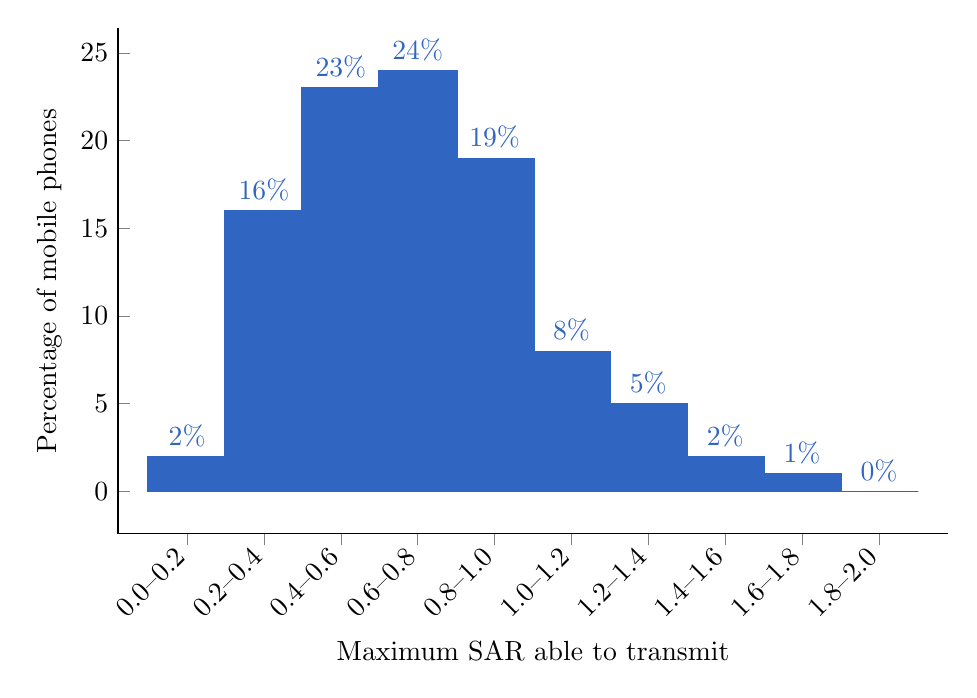
\begin{tikzpicture}
  \begin{axis}[
          ybar=-1cm,
          axis x line*=bottom,
          axis y line*=left,
          bar width=1cm,
          xlabel near ticks,
          height=8cm, width=\textwidth,
          ylabel={Percentage of mobile phones},
          xlabel={Maximum SAR able to transmit},
          symbolic x coords={0.0--0.2,0.2--0.4,0.4--0.6,0.6--0.8,0.8--1.0,1.0--1.2,1.2--1.4,1.4--1.6,1.6--1.8,1.8--2.0},
          x tick label style={rotate=45, anchor=east, align=left},
          nodes near coords={\pgfmathprintnumber\pgfplotspointmeta\%},
          nodes near coords align={vertical}      
          ]
          \addplot[hous,fill]  coordinates {(0.0--0.2,2)};
          \addplot[hous,fill]  coordinates {(0.2--0.4,16)};
          \addplot[hous,fill]  coordinates {(0.4--0.6,23)};
          \addplot[hous,fill]  coordinates {(0.6--0.8,24)};
          \addplot[hous,fill]  coordinates {(0.8--1.0,19)};
          \addplot[hous,fill]  coordinates {(1.0--1.2,8)};
          \addplot[hous,fill]  coordinates {(1.2--1.4,5)};
          \addplot[hous,fill]  coordinates {(1.4--1.6,2)};
          \addplot[hous,fill]  coordinates {(1.6--1.8,1)};
          \addplot[hous,fill]  coordinates {(1.8--2.0,0)};
      \end{axis}
  \end{tikzpicture}
  \caption{Distribution of how many phones belong to a certain SAR interval. Upper boundary not included.}
  \label{chart:germanDatabase}
\end{figure}


\subsubsection{Whole Body Specific Absorption Rate}
The position of the phone relative to the user's body is however unknown. 
Some users will be calling and therefore probably holding their phone next to their ear while others are using other services like browsing the web. 
This would result in different types of localized values. To be able to give an average SAR based on all active users, the whole body SAR will be used.
For this reason formula \ref{eq:overallSARwb} expects that the specific absorption rate is expressed for the entire body instead of localized $SAR^{head}_{10g}$.
The conversion factors for Duke from the Virtual Family will be used again as it was already the case in \ref{sub:convertDLtosarwb}. 
The constant to convert \gls{UL} exposure to $SAR^{wb,myUE}_{10g}$
for WiFi is defined to be 0.0070 $\frac{W/kg}{W}$ \cite{J22_plets2015joint} which leads to eq. \ref{eq:ulToSar}.

\begin{equation} 
SAR^{wb,myUE}_{10g} \left[\frac{W}{kg}\right] = 0.0070 \left[\frac{W/kg}{W}\right] * P_{tx}^{UE} [W]
\label{eq:ulToSar}
\end{equation}

The power of the \gls{UE} can be calculated using equation \ref{eq:powerUE} \cite{J22_plets2015joint}.
\begin{equation} 
P_{tx}^{UE} = \big\{P_{max} [dBm] , P_{pusch} [dBm] + \alpha * PL [dB] + 10log(M) + \sigma \big\}
\label{eq:powerUE}
\end{equation}

$P_{max}$ is the maximum allowed transmission power by \gls{UE} for LTE, defined at 23 dBm. 
However, this is the worst case and the actual used power is uselly mutch lower thanks to power control.
$P_{pusch}$ is the required received power at the
\gls{UABS} and will be advertised by the base station over the \gls{pusch}. This research will use a
$P_{pusch}$ of -120 dBm. 
$\alpha$ is the path loss compensation factor where 
$\alpha$ must equal \{0,0.4,0.5,0.6,0.7,0.8,0.9,1\}. An $\alpha$ set to 
zero indicates there is no path loss compensation \cite{J32,J33}.
For this document, full pathloss compensation will be used with an $\alpha$ equal to one.
For the 20-MHz
channel used in this paper, $M$ will be set to 100; indicating the number of  used resource blocks by \gls{pusch} \cite{J22_plets2015joint}.
Finally, we have $\sigma$
 as the correnction factor and is set to zero. Other possible values are \{-1, 0, 1, 3\} \cite{J22_plets2015joint,J32}.
 The presented values can be found in the overview given in table \ref{table:defaultconf}.

\section{Microstrip Patch Antenna}
\subsection{Design of  a Microstrip Patch Antenna}
\label{sub:definingAntenna}
A microstrip patch antenna is chosen because it allows easy production but more important, it has a low weight 
and has a thin profile causing it to be very aerodynamic which is useful when attaching it to a drone \cite{J13_microstripadvantages}.

The dimensions of the antenna depend on the frequency it is operating at and the characteristics of the used substrate.
The antenna will be radiating at a center frequency $f_0$ of 2.6 GHz. Each substrate has a \gls{dielectric constant} $\epsilon_r$ representing 
the permittivity of the substrate that depends on the used material.
Substrates with a high \gls{dielectric constant} and low height 
reduce the dimensions of the antenna
while a lower \gls{dielectric constant} with a high height improves antenna performance \cite{J14_antennadesign,J15_antennadesign}. 
In this document, a substrate like glass 
is chosen because of the higher \gls{dielectric constant} of $\epsilon_r = 4.4$ compared to materials like Teflon with only a dielectric 
constant of $\epsilon_r = 2.2$ \cite{J14_antennadesign}. 
Doing this in combination with an antenna height of 2.87 mm will decrease the dimensions of the entire antenna surface.
This comes in handy since drones only have limited space available.

\begin{table}[h!]
\centering
\begin{tabular}{|l|c|l|}
\hline
 Description            & Symbol          & Value         \\    \hline
 Center frequency       & $f_0$           & 2600 Hz       \\ 
 Dielectric constant    & $\epsilon_r$    & 4.4         \\ 
 Height of the substrate & $h$             & 0.00287 m    \\ \hline
\end{tabular}
\caption{Overview of the configuration parameters.}
\label{table:antennaparas}
\end{table}

The dimensions of the radiating patch can be calculated with the formulas from \cite{J14_antennadesign} and \cite{J15_antennadesign}
using the defined values from table \ref{table:antennaparas}. In that way, the width of the patch $W_{p}$ is calculated using formula \ref{eq:antennawidth}.

\begin{equation} 
W_{p} [m] = \frac{C [m/s]}{2*f_0 [Hz]}*\sqrt{\frac{\epsilon_r+1}{2}}
\label{eq:antennawidth}
\end{equation}
With $C$ being the speed of light, $f_0$ the center frequency of 2600 MHz and a \gls{dielectric constant} $\epsilon_r$ of 4.4, the width of the patch becomes 35.09 mm.

In order to find the length of the radiating patch, some other values need to be determined first. Formula \ref{eq:epsilonreff} will
calculate the effective \gls{dielectric constant} ($\epsilon_{reff}$).
\begin{equation} 
\epsilon_{reff} = \frac{\epsilon_r+1}{2}+  \frac{\epsilon_r-1}{2} * \left(1+12*\frac{h [m]}{W_{p} [m] }\right)^{-\frac{1}{2}}
\label{eq:epsilonreff}
\end{equation}
This formula requires the width found in the previous formula along with the \gls{dielectric constant} and substrate height from table \ref{table:antennaparas}.
This will result in a $\epsilon_{reff}$ of 3.91.

\begin{equation} 
L_{eff} [m] = \frac{C [m/s]}{2*f_0 [Hz]}*\sqrt{\epsilon_{reff}}
\label{eq:leff}
\end{equation}
Now formula \ref{eq:leff} can be used to calculate the effective length ($L_{eff}$), resulting in 29.16 mm.

\begin{equation} 
\Delta L [m]= 0.412*h*\frac{(\epsilon_{reff}+0.3)\left(\frac{W_{p} [m]}{h [m]}+0.264\right)}{\left(\epsilon_{reff}-0.258\right)\left(\frac{W_{p} [m]}{h [m]}+0.8\right)}
\label{eq:lenghtextension}
\end{equation}
Eventually, the length extension is found with formula \ref{eq:lenghtextension} by substituting the values from above.
Doing so determines that the $\Delta L$ equals 1.3071 mm.

Finally, the length of the patch can be calculated using the expression \ref{eq:realLenght}
\begin{equation} 
L_p [m]= L_{eff} [m] - 2 * \Delta L [m]
\label{eq:realLenght}
\end{equation}
The length $L_p$ results in 26.55 mm.

The dimensions of the radiation patch are now known. The only remaining questions are the dimensions of the ground plane and dielectric substrate to which the 
radiation patch is attached. The transmission line model is in fact only applicable for an infinite ground plane but it has been proven that similar results
can be achieved if the ground plane's dimensions are bigger than the patch by approximately 6 times the height of the dielectric substrate \cite{J14_antennadesign,J15_antennadesign}.

\begin{equation} 
L_{g} [m] = 6 * h [m] + L_p [m]
\end{equation}
\begin{equation} 
W_{g} [m] = 6 * h [m] + W_p [m]
\end{equation}
Therefore, the length of the ground plane $L_{g}$ should be at least 0.0438 m and the width $W_{g}$ at least 0.0524 m.
A schematic overview of how the antenna will look like is given in figure \ref{fig:antennadesign}.
\begin{figure}[h!]
\centering
  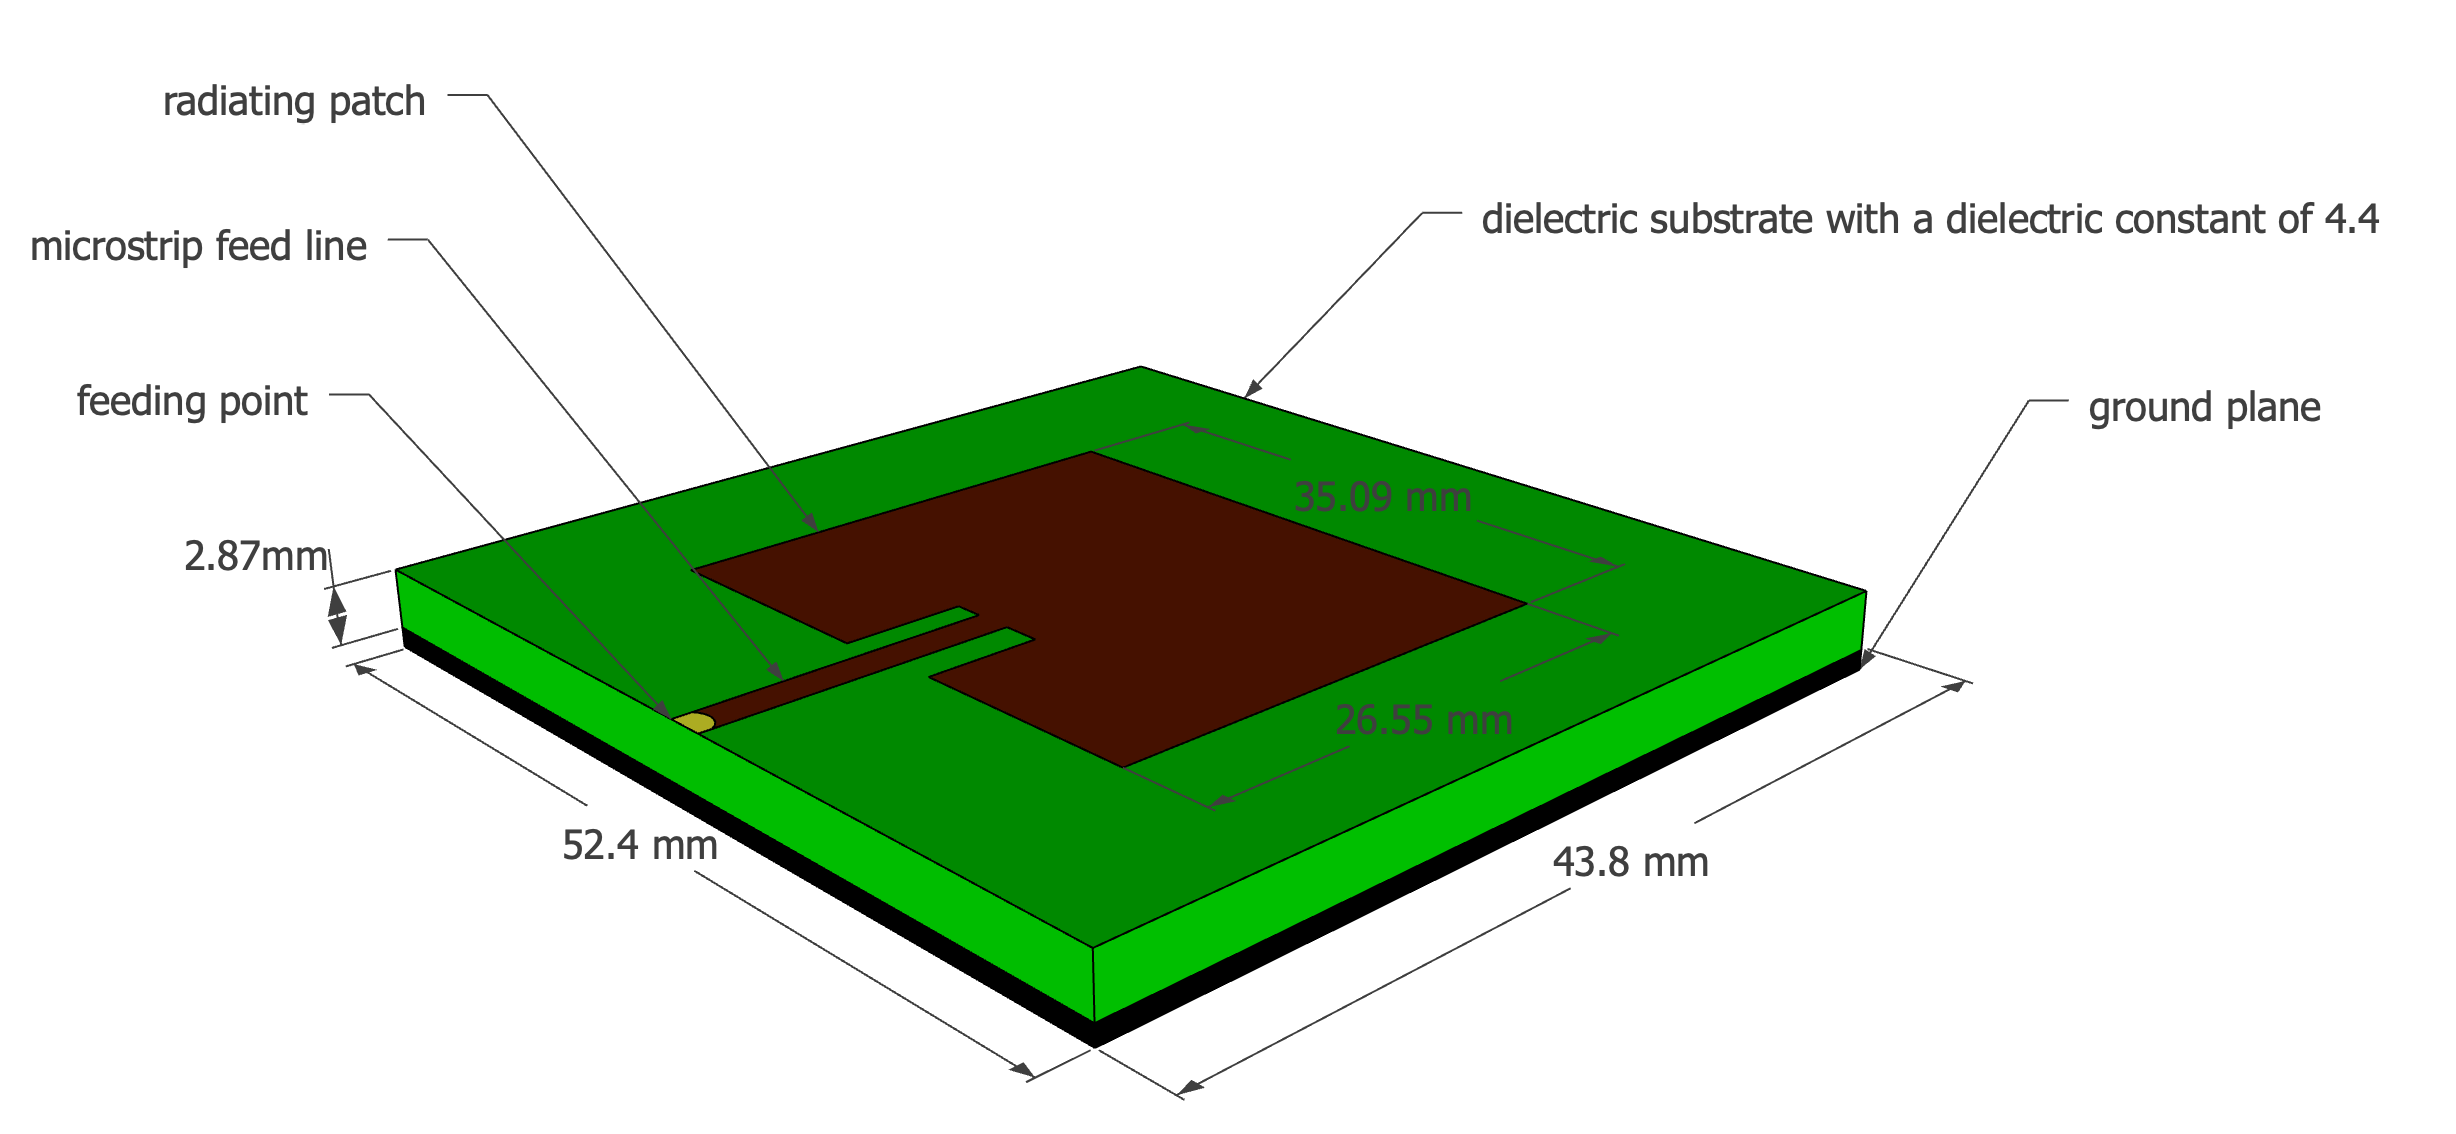
\includegraphics[width=\textwidth]{../images/MicrostripAntenna.png}
  \caption{Design of the microstrip patch antenna.}
  \label{fig:antennadesign}
\end{figure}

\subsection{Radiation Pattern}
Matlab is able to generate the radiation pattern for this microstrip patch antenna.
The code in  listing \ref{c:mathlabradpattern} starts by defining the dielectric substrate which will be glass with a \gls{dielectric constant}
of 4.4 and a height of 0.00287 m. Thereafter, the microstrip patch antenna is generated with the \verb|width| and \verb|length| being the dimensions
of the radiation patch and the \verb|GroundPlaneLength| and \verb|GroundPlaneWidth| the dimensions of the ground plane and dielectric substrate.
The \verb|FeedOffset| is the relative offset from the center where the radio frequency power is fed to the radiating patch which will here be
at the edge. This is in figure \ref{fig:antennadesign} indicated with a yellow dot. At last, the \verb|dielectric|-object is substituted into the 
\verb|patchMicrostripInsetfed|-object.

Generating the pattern is done with the \verb|pattern|-command. The first value is the \\ \verb|patchMicrostripInsetfed|-object followed by the frequency
at which the antenna will be operating. Optionally, an azimuth value can be parsed like in line 7 and 8 where 90 and 0 relatively stand for the H-plane and E-plane.

\begin{listing}[h!]
\begin{minted}[frame=single,framesep=10pt,xleftmargin=20pt,linenos]{c}
d = dielectric("Name",'glass',"Thickness",0.00287,"EpsilonR",4.4)
p = patchMicrostripInsetfed("Width",0.0351,"Length",0.02655,
    "GroundPlaneLength",0.0438,"GroundPlaneWidth",0.O524,
    "FeedOffset",[-0.021885 0],"Substrate", d)

pattern(p,2.6e9, "CoordinateSystem", 'polar', "Normalize",true)
pattern(p,2.6e9, 90, 0:10:360, 
        "CoordinateSystem", 'polar', "Normalize",true)
pattern(p,2.6e9, 0, 0:10:360, 
        "CoordinateSystem", 'polar', "Normalize",true)
\end{minted}
\caption{Matlab code to generate the radiation patterns for the microstrip patch antenna.}
\label{c:mathlabradpattern}
\end{listing}

Running the configuration from listing \ref{c:mathlabradpattern} will generate the radiation pattern from figure \ref{radpattern2}.
When running the same configuration for a slightly bigger square ground plane with an edge of 0.060 m, the radiation pattern from \ref{radpattern1} is
achieved. Both radiation patterns show an aperture angle of approximately 90°. It becomes clear that the radiation pattern from figure \ref{radpattern2} has a higher attenuation in the direction it is not facing compared to
the radiation pattern of figure \ref{radpattern1}. If it is assumed that drones fly lower than some users are positioned in some buildings, the pattern of 
\ref{radpattern1} would be a better approach. 
However, for the continuation of this master dissertation, the radiation pattern from figure \ref{radpattern2} 
will be used since this antenna is the smallest
and therefore most suitable to attach to the limited space available under a drone. 
An more extensive comparison between different radiation patterns is out of the scope of this master dissertation. 
A data sheet of the exact values from both radiation patterns can be
found in appendix \ref{ch:radpattern}.


\begin{figure}[!htb]
\subfloat[3D model of the entire pattern]{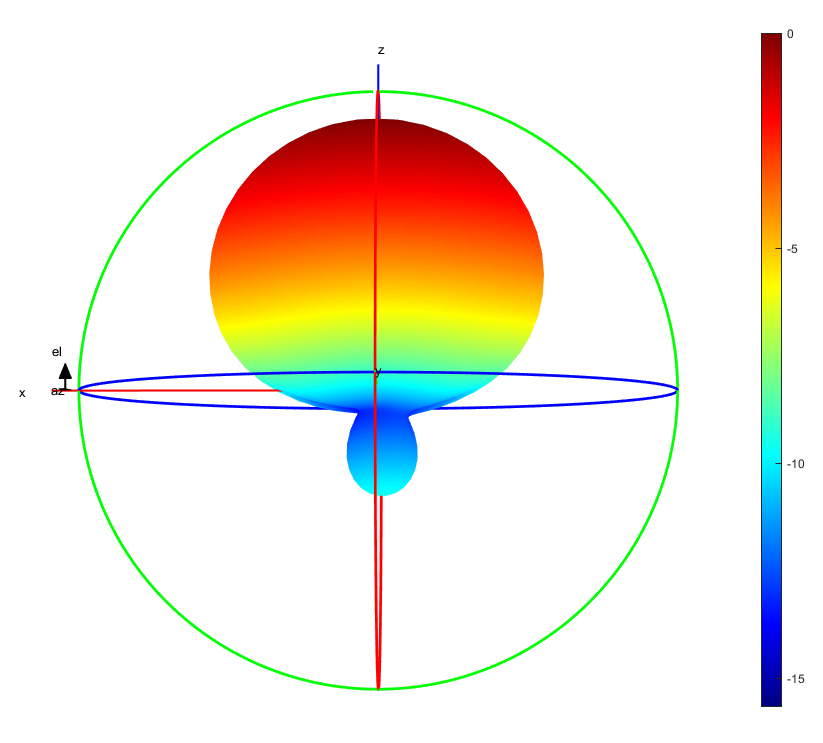
\includegraphics[height=2in]{../images/pattern2/pattern.png}}
\subfloat[2D model of the E-plane]{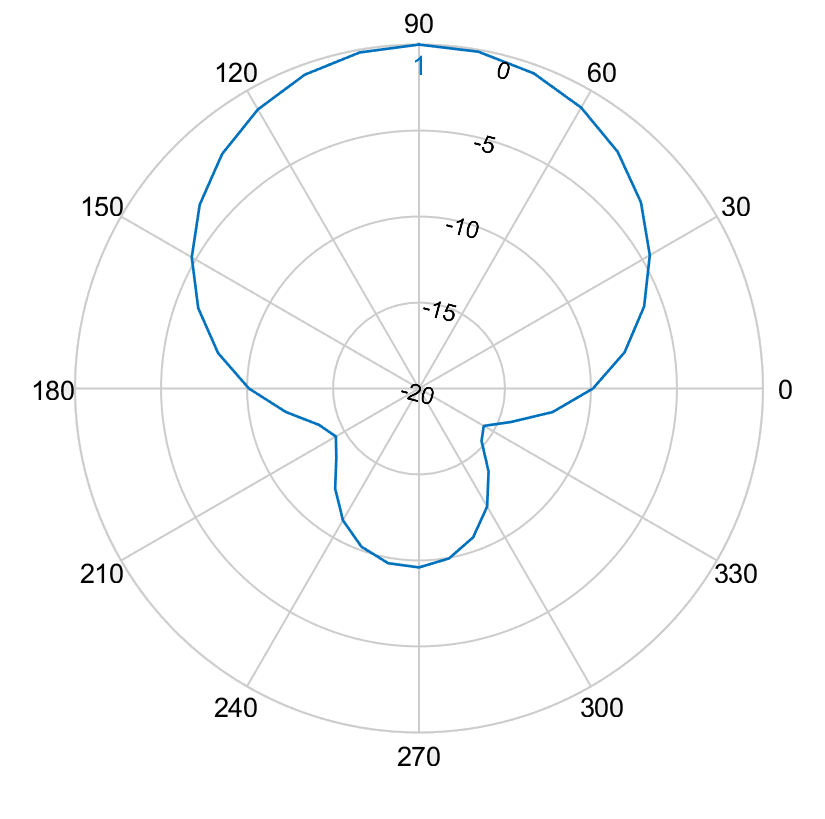
\includegraphics[height=2in]{../images/pattern2/ep.png}}
\subfloat[2D model of the H-plane]{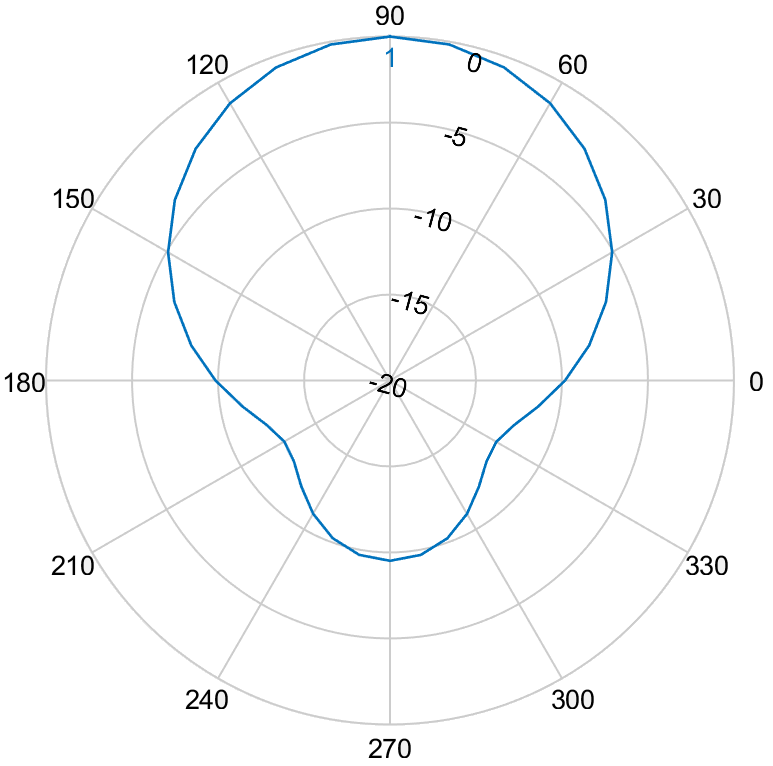
\includegraphics[height=2in]{../images/pattern2/hp.png}}
\caption{Radiation pattern 1 (in dBi) with the configuration as described above.}
  \label{radpattern2}
\end{figure}

\begin{figure}[!htb]
\subfloat[3D model of the entire pattern]{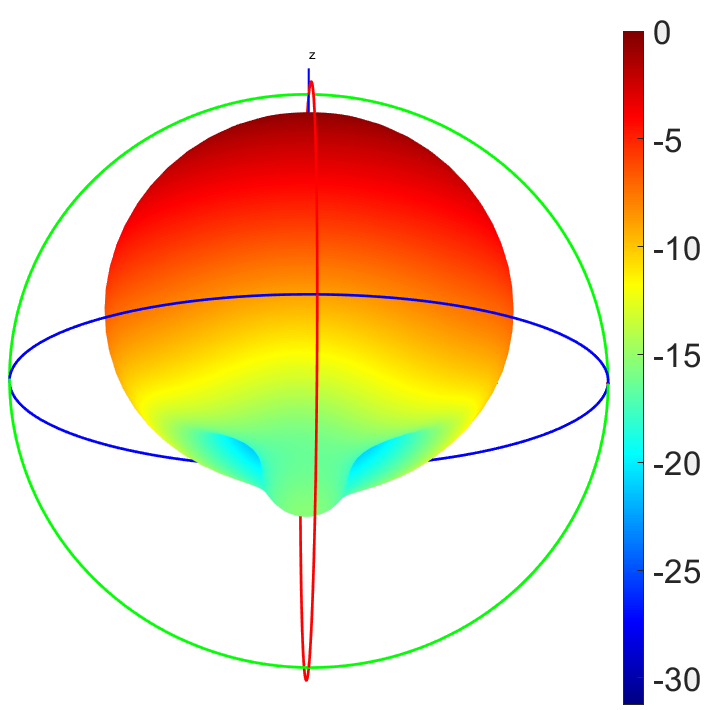
\includegraphics[height=2in]{../images/pattern1/radiationPattern3D.png}}
\subfloat[2D model of the E-plane]{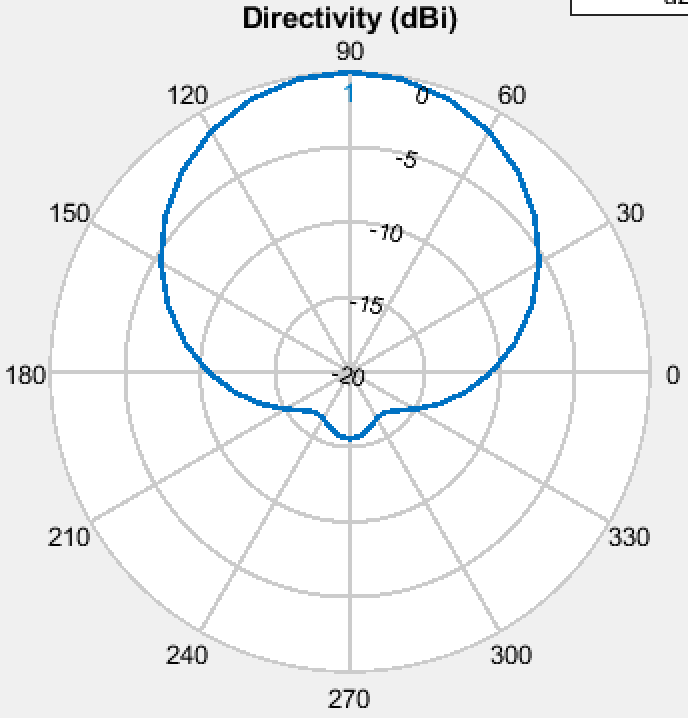
\includegraphics[height=2in]{../images/pattern1/ep.png}}
\subfloat[2D model of the H-plane]{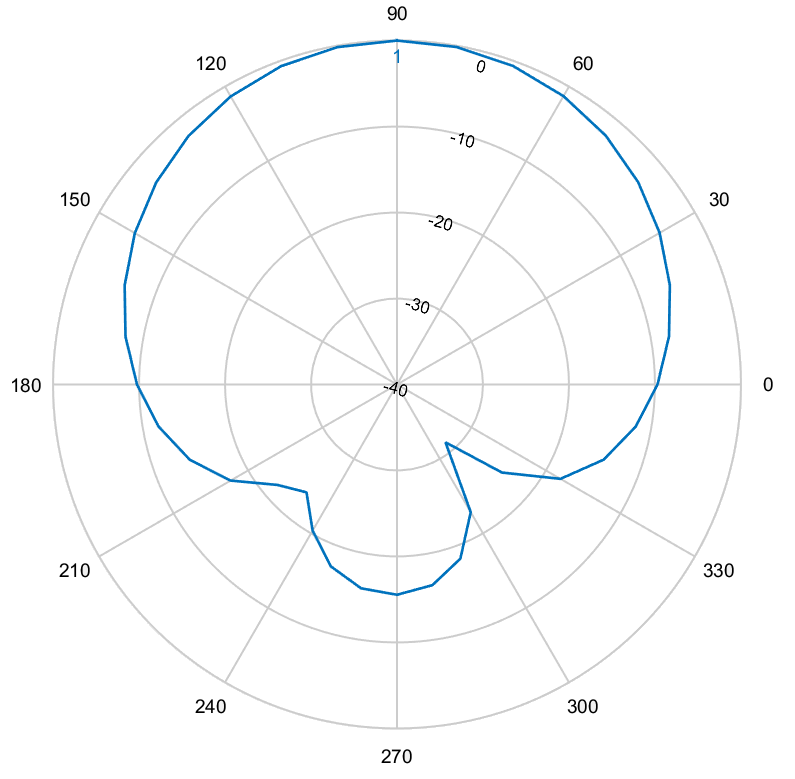
\includegraphics[height=2in]{../images/pattern1/hp.png}}
\caption{Radiation pattern 2 (in dBi) which is generated with a groundplane of 0.06m by 0.06m. }
 \label{radpattern1}
\end{figure}

\section{Optimizing the Network}
\label{sec:methodology:optimizingTheNetwork}

\gls{UAV}s can remain in the air for only a limited time, which is certainly 
the case when also an antenna needs to be connected to the battery of his carrier. It is therefore
interesting to not only consider electromagnetic exposure of the user but also the power consumption that comes with it. 
However, an increasing transmission power of an antenna comes with an increasing electromagnetic exposure, this is not the case considering
both values for an entire network. In fact, the authors from \cite{J1}  prove that both become inversely equivalent.

The reason the network behaves like this is because it is often cheaper to increase the exposure of an already active base station 
than activating a new one. 
As an example, imagine there is a new user who can either be covered by activating a nearby base station or 
by an already active base station a little further away. When this user is in a power consumption optimized network, 
the already active base station will increase its power level because that will be cheaper than activating a new base station. 
Users close by will thus experience a higher electromagnetic exposure. On the other hand, if the user would have been in an exposure 
optimized network, the nearby base station which was offline would be activated at a lower power level. So the electromagnetic 
exposure will also be lower but by activating a new base station, the overall power consumption increases.

This results in conflicting requirements. An optimization strategy that 
optimizes towards either electromagnetic exposure or total power consumption is given in \ref{eq:fitnessfunction} and is
based on the fitness function described in \cite{J1}.

\begin{equation} 
f = w * \left(1 - \frac{E_m}{E_{max}}\right) + (1 - w)*\left(1 - \frac{P}{P_{max}}\right) * 100
\label{eq:fitnessfunction}
\end{equation}

Formula \ref{eq:fitnessfunction} returns a fitness value which represents the performance of the entire network. Users are connected to different \gls{UABS}s and each time a fitness value is 
calculated. The user will eventually be connected to the drone that results in the highest fitness value. 
This is repeated for each user. This process is explained in detail in section \ref{sec:implementation:deploymenttool}.
$w$ is the importance factor of electromagnetic exposure ranging from 0 to 1, boundaries included. A $w$ set to zero means that electromagnetic 
exposure is not important. Such a network will therefore be called a \gls{PwrC Opt}. 
Likewise, a $w$ set to one means that minimizing exposure is top priority and will result in an \gls{Exp Opt}. $P_{max}$ is the power consumption of all \gls{UABS}s, both active and inactive, when radiating at the highest possible level 
while $P$ is the effective power used by the current designed network. 
This will be the power required for the flying drones themselves and their antenna.
$E_m$ will be the weighted exposure of the average user for the current designed network and $E_{max}$ the weighted average of electromagnetic exposure when all antennae are at their highest power level.

When optimizing the network, it is not only important to consider the average exposure of all users, but also to limit high extremes \cite{J1}. 
In formula \ref{eq:em} a weighted average of exposure will be found by not only considering the median but also the 95 percentile of all users' DL exposure.
Since both values are considered to have equal importance, the weight factors $w_1$ and $w_2$ will both have an equal importance of 50\%. 

\begin{equation} 
E_m = \frac{w_1 * E_{50} + w_2 * E_{95}}{w_1 + w_2}
\label{eq:em}
\end{equation}
%\textcolor{red}{todo: in J1 is dit gedetailleerder uitgeschreven. Mogelijk om hier wat extra over te schrijven.}


\section{Simulation Tool}

\subsection{Implementation of the Deployment Tool}
\label{sec:implementation:deploymenttool}
\subsubsection{Main Algorithm}

Calculating electromagnetic exposure requires knowledge about the area. 
For instance, the position of \gls{UABS}s needs to be known but also  other variables like
 the used transmission power and the distances between antennae.

The WAVES research group at Ghent University has developed a capacity based deployment tool for disaster scenarios with the aid of UAVs \cite{J2}.
The idea of this UAV-aided emergency network is that in case of a disaster, the existing terrestrial network might be damaged and will not be able 
to handle all users who are trying to reconnect to the backbone network. 
The tool makes a fast deployable network possible by attaching femtocells to UAVs, so-called \gls{UABS}s.
The tool will orchestrate the \gls{UABS}s over the disaster area by describing a fully configured network.
This tool is thus a suitable starting point and works as follows:

The deployment tool will try to calculate the optimal placement for each \gls{UABS} and requires therefore a description of the area where the UAV-aided network needs to 
be deployed. This is done with the use of so-called shape files. These files contain three dimensional descriptions of the buildings present in the area and are
key values in approaching results as realistic as possible. Furthermore, the tool also requires a configuration file containing technical specifications of the type of \gls{UABS} that is being used. 
The tool will thereafter randomly distribute users over the area and assigns a certain bitrate to them (figure \ref{fig:userdistribution}). If a user is indoor, the height of the user will be estimated 
at hal the height of the building. The height \gls{UE} itself will be 1.5 metres above the floor. 

\begin{figure}[h!]
\centering
 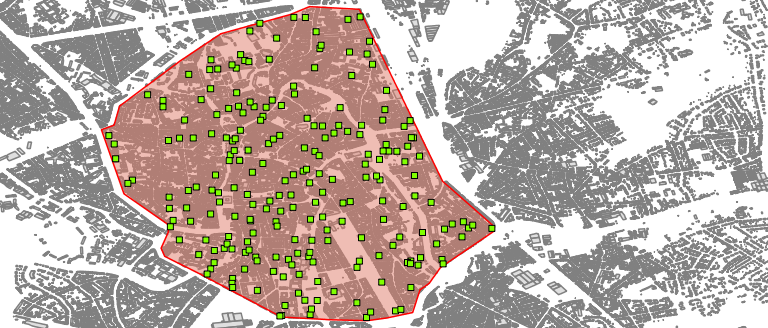
\includegraphics[width=.85\textwidth]{../images/cityCenterGhentUserDistributionB.png}
  \caption{Example of how users are randomly distributed over the city centre of Ghent.}
  \label{fig:userdistribution}
\end{figure}

In a second phase, the optimal position for each \gls{UABS} is calculated. This is done by trying to locate a \gls{UABS} above each active user. Two options are possible.
If a fixed flying height is defined, a \gls{UABS} is placed above each user at the given height, unless a building is obstructing its location. Then, no base station will be located above that user.
Alternatively to the fixed flying height, a flying margin can be defined which represents the distance between the outdoor user and  the drone.
If the user is inside, this margin will be measured between the drone and the rooftop of that building.
The latter is only allowed if the suggested height remains below the given maximum allowed height.

Thereafter, the decision algorithm calculates which users should be connected to which \gls{UABS}s. 
These decisions are based on the specified optimization strategy. For this master dissertation,
this will either be power consumption optimized or exposure optimized.

In the final state, unused \gls{UABS}s are removed and the capacity of the facility is checked. 
If the number of active drones would exceed this capacity, \gls{UABS}s will be sorted based on the number of 
users they cover. Thereafter, drones with too few users are removed so that all the active drones could be stored in the facility.
The flowchart of the main algorithm is given in figure \ref{fig:mainflow}.
\begin{figure}[h!]
\centering
 \includegraphics[width=\textwidth]{../images/mainflow.png}
  \caption{Flowchart of the main algorithm.}
  \label{fig:mainflow}
\end{figure}

\subsubsection{Decision Algorithm}

\noindent
\begin{minipage}{0.6\textwidth}% adapt widths of minipages to your needs
  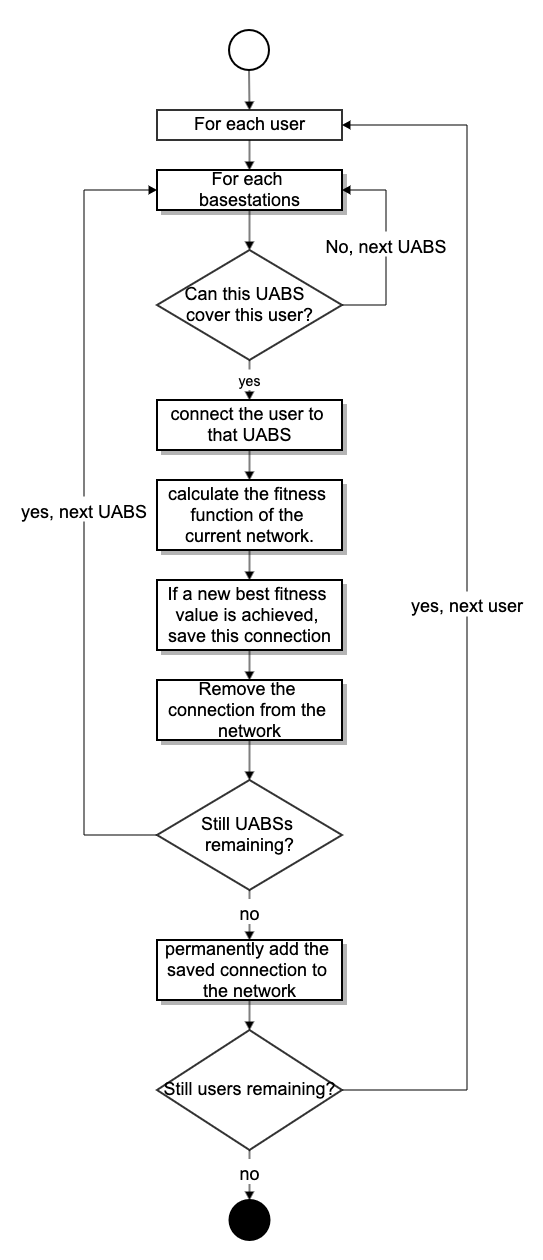
\includegraphics[width=\textwidth]{../images/decisionAlgoFlowChart.png}
  \captionof{figure}{Flowchart of the decision algorithm.}
  \label{fig:decisionAlgoFlowChart}
\end{minipage}%
\begin{minipage}{0.4\textwidth}\vspace{-120pt}%
Solving the network is done by the decision algorithm and starts by calculating the path loss
between the different users and thereafter between users and \gls{UABS}s.
Thereafter, the tool iterates over each user and tries to connect that user to each \gls{UABS}. This connection is not always possible. A \gls{UABS} might be saturated with users and 
will not be able to cover yet another one or maybe the user is so far away that in order to cover that user, the \gls{UABS} would have to exceed its maximum allowed input power.
However, if a connection is possible, the user will be connected to that \gls{UABS} and the fitness function from section \ref{sec:methodology:optimizingTheNetwork} is applied. 
This is repeated for each \gls{UABS}. Only the connection which results in the best fitness value for the entire network will be used. 
Doing so will make sure that, given the currently designed network, the user is optimized. In other words, each user is optimized and 
not the entire network. It is however assumed that the average network will be optimized as well.
Thereafter, the tool shifts to the next user. 
When the last user has been processed, the network is fully designed for an unlimited number of drones and the result is returned to the main algorithm for further processing.
The flowchart of this algorithm is given in figure \ref{fig:decisionAlgoFlowChart}.
\end{minipage}

\FloatBarrier
\subsection{Implementation of the Radiation Pattern}
\label{subsec:implementationradpat}

Originally, the deployment tool  did not considered attenuation. 
Therefore, the radiation from the antenna attached to the \gls{UAV} 
was equal in each direction. Such a fictional antenna is called an \gls{isotropicradiator}. 
Thus the tool has been extended in order 
to support several types of antennae by introducing new parameter like attenuation and direction.
Doing so allows any type of antennae which is fully configurable in any given orientation.
This configuration is done with the usage of an XML-file which will apply to all \gls{UABS}s in the network.
An \gls{isotropicradiator} is still supported by returning 
a zero value when the attenuation is requested.

The orientation is done using two values called `downtilt' and `north offset'. The first value
defines the downtilt angle under which the antenna is pointing. A downtilt angle of zero degrees is perfectly horizontal and 
an antenna with a downtilt angle of \ang{90} will be pointing straight to the ground.
This parameter only supports positive values ranging from \ang{0} to \ang{360} (upper boundary not included). An antenna pointing to the sky would therefore require a value of \ang{270}.
The second value, the north offset, defines the azimuth orientation of the drone. The value given to this parameter indicates the offset between the north
and the horizontal direction to which the antenna should be pointing at. The value once again ranges from \ang{0} to \ang{360} with the upper boundary not included. The
angle is calculated in counterclockwise orientation. For instance, a north offset of \ang{270} will let the \gls{UABS} point to the east.  
An example is given in figure \ref{fig:droneOrientations} where
fig. \ref{fig:droneOrientations}.a shows a \gls{UAV} that performs a horizontal movement with a north offset of \ang{90}.
The antenna attached to the \gls{UAV} in fig. \ref{fig:droneOrientations}.b performs a downtilt movement of \ang{90}.



\begin{figure}[!htb]
\subfloat[north offset of \ang{90}]{ 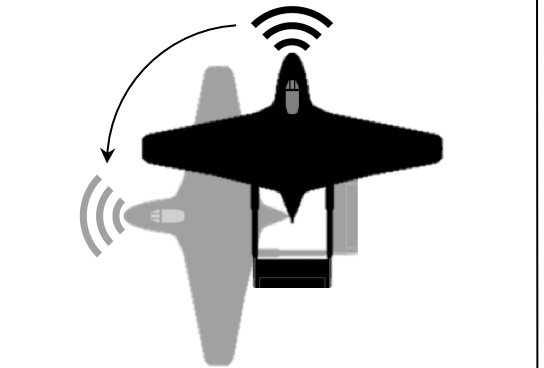
\includegraphics[width=\textwidth*1/3]{../images/droneOrientations_no.png}}
  \subfloat[downtilt of \ang{90}]{

    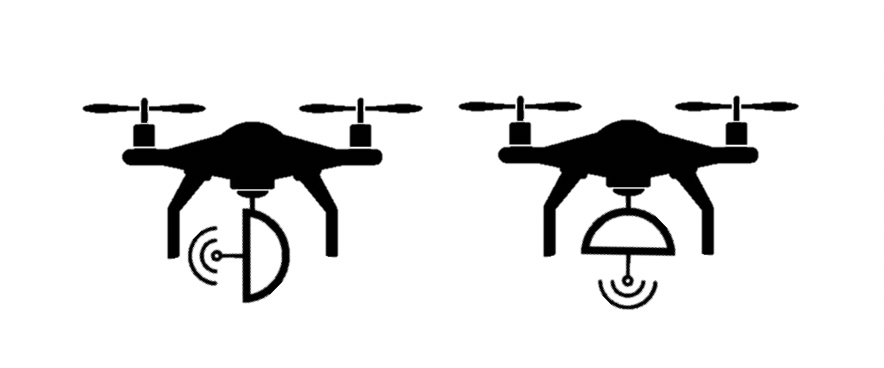
\includegraphics[width=\textwidth*2/3]{../images/droneOrientations_dt.png}
    }
 \caption{Illustration of the two possible movements. The \gls{UAV} in fig. (a) is a top view while the \gls{UAV} in fig. (b) is a side view. }
  \label{fig:droneOrientations}
\end{figure}

Thereafter, the normalized radiation pattern is supplied to the tool, the actual pattern is three dimensional. To simplify this,
slices perpendicular to the az-axis are extracted. These are indicated in figure \ref{fig:slicesOfPattern} with azimuth cuts. With
an angle of \ang{90} four slices are achieved, each consisting out of elevation cuts. The intersection of an elevation and azimuth plane 
corresponds with a certain attenuation which is fed to the tool. Figure \ref{fig:slicesOfPattern} shows only 3 elevation planes. The radiation pattern used in the tool 
has an attenuation every \ang{10}. In other words, a slice consists of 19 values ranging from \ang{0} to \ang{180} (boundaries included).
\begin{figure}[H]
\centering
  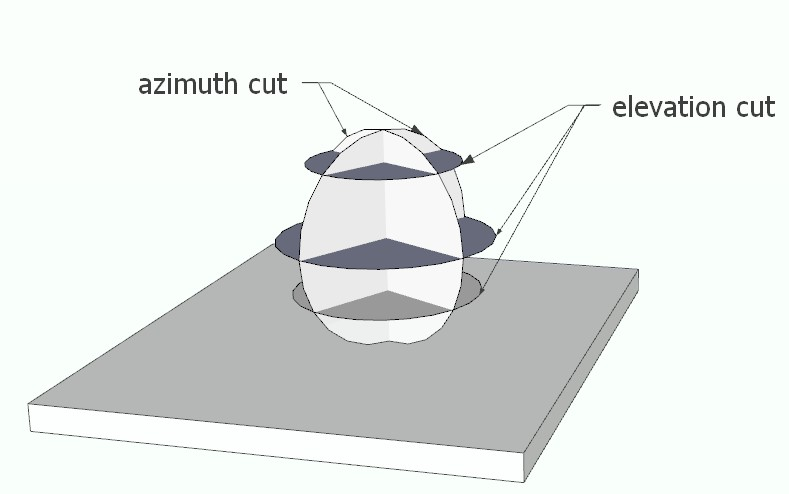
\includegraphics[width=\textwidth/10*6]{../images/3Dimages/slicesOfPattern.jpg}
  \caption{Schematic example of slices in a radiation pattern.}
  \label{fig:slicesOfPattern}
\end{figure}

The number of required slices depends on the complexity of the radiation pattern. For symmetrical radiation patterns, like 
in figure \ref{radpattern2} and \ref{radpattern1}, two azimuth cuts perpendicular to each other
are definitely sufficient. This is also illustrated in figure \ref{fig:slicesOfPattern} where two azimuth planes are shown and that, once cut, will result in four slices.
However, this might not be the case for radiation patterns with a more complex structure containing several  
side lobs. To tackle this issue, more azimuth-slices can be defined for increased precision. Each slice should however contain an equal amount 
of elevation slices.  A concrete example of a configuration file can be found in appendix \ref{ch:radpatexampleconfig}.
 
When the attenuation of a user from a certain \gls{UABS} needs to be known, the elevation and azimuth angles between the user and the antenna's direction 
should be calculated. 
Figure \ref{fig:globe} represents a radiation pattern with the black dot indicating the user whose attenuation needs to be calculated.
The small black lines represent azimuth and elevation planes. 
The tool knows the exact attenuation only at the intersection of those lines. 
The chance that a user is positioned at such an intersection is very small. Therefore, the attenuation for the requested point has to be estimated using bilinear interpolation.
First, the attenuation is estimated at the intersection of the red and orange line using linear interpolation on the horizontal axis with the known values at the end of the red line. 
The same is done for the orange-green intersection using the known values at the end of the green line. Finally, linear interpolation
is applied to the y-axis for the black dot on the orange line using the estimated values at the end of the orange line.

\begin{figure}[H]
\centering
  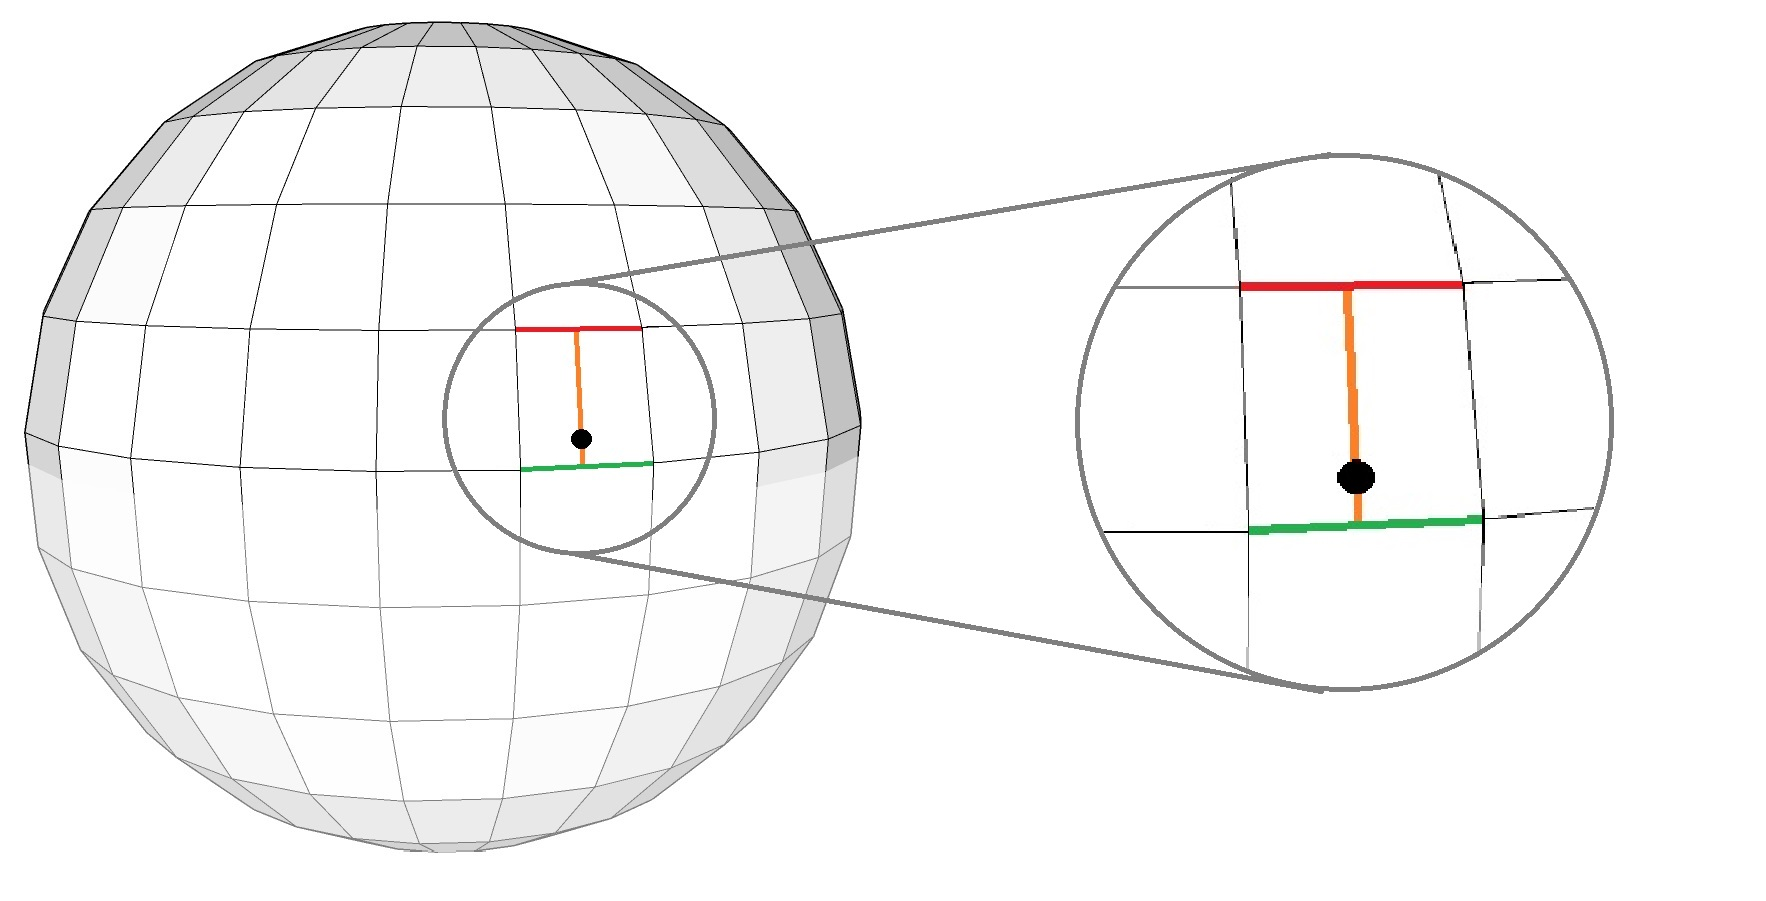
\includegraphics[width=\textwidth/3*2]{../images/3Dimages/globev2.jpg}
  \caption{Schematic example of how bilinear interpolation works.}
  \label{fig:globe}
\end{figure}

\subsection{Performance Improvement}
\subsubsection{Calculating Path Loss}
The path loss is required by several formulas. For instance, the formula that decides whether a \gls{UABS} is feasible for a certain 
user makes use of this parameter but also the calculations for the downlink electromagnetic 
exposure require this value to be known. The formulas for the whole body $SAR_{10g}$ require not only the path loss between the user
and all \gls{UABS}s but even the path loss between users themselves. These path loss calculations are based on the Walfish-Ikegami 
model that causes a high computational load.  The calculation between two points is completely independent of any other calculation between any 
other points and is therefore a suitable candidate to multithread.
 The deployment tool creates two thread pools.
The first pool creates a thread for each user where each thread calculates the path loss between the user assigned to him and all possible \gls{UABS}s,
causing a time complexity of $n^2$.
Each user stores all path losses between himself and any other \gls{UABS}. This results therefore in a total space complexity of $n^2$.
When all users are finished, the thread pool is shut down and the second one is created for the same calculations but between users.
The pool will, just like the previous, create threads for each user but there is an important difference.
When a certain user calculates the path loss to another user, this path loss also applies for the other direction. The tool saves time by calculating the path loss only 
once and stores the path loss at both users. It is therefore sufficient that a given user only calculates path losses of users at his right side, since the other path losses will 
be calculated by the users on his left. This results in a time complexity of only $n(\frac{n}{2})$. When the last user finishes his thread, all users know the path loss of all other users causing 
a space complexity of $n(n-1)$.
% eventueel nog over concurrent hashmap

\subsubsection{Limiting Antenna Searching}
The user needs to be connected to the `best' base station. To identify this best \gls{UABS}, the user should be connected 
to each base station and the value of the fitness function presented in equation \ref{eq:fitnessfunction} has to be evaluated. 
The connection that resulted in the best fitness function
will be added to the solution. This process is repeated for each user but can further be improved. 
A user will likely be connected to either the
\gls{UABS} directly above him or to a \gls{UABS} in the direct neighbourhood. 
Time complexity can thus be improved by not considering drones outside a certain radius.
An ideal data structure for neighbourhood-search with geographical coordinates is a KD-tree \cite{J27,J28}. 
This data structure  is described by Bentley in \cite{J29}  and is based on a binary tree, optimal for objects consisting out of 
multiple keys.
Each node in this tree is associated with a certain dimension and will split the hyperplane over exact one dimension.
In this case, the x and y coordinate will be used in a 2D-tree (k=2) like in figure \ref{fig:exampleKDtree}.

\begin{figure}[]
  \centering
  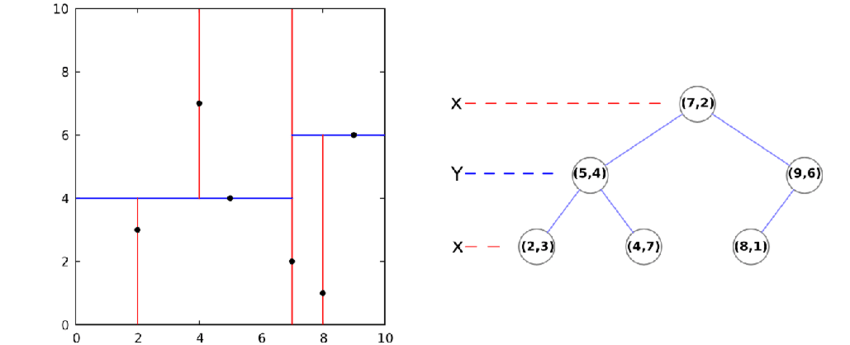
\includegraphics[width=\textwidth/10*8]{../images/Example-of-a-2D-k-d-tree.png}
  \caption{Example of a KD-tree in two dimensions.}
  \label{fig:exampleKDtree}
\end{figure}

The length of  the connections is investigated to define a proper cut-off radius.
The investigated network is a power consumption optimized network with an \gls{isotropicradiator} because this 
configuration will result in the biggest cell sizes due to the absence of attenuation in the antenna. 
Figure \ref{chart:distances} shows that for small networks with 50 users, 78\% of the connections
are less than 100 metres. The other 22\% are situated between 100 and 400 metres and decrease logarithmically.
For bigger networks with 600 users, 57\% of the connections is less than 100 metres. The remaining 43\%
of the connections are situated between 100 and 500 metres. No significant percentage of connections longer than 500 metre
were recorded for either cases.
The percentage of  connections less than 100 metres will even be higher when using exposure optimized networks 
and/or microstrip patch antennae.
In this case the choice was made to only consider \gls{UABS}s within a radius of half a kilometre which is believed 
to have a sufficient safety margin. The rare connections that would have exceeded this radius would not contribute much to 
the average values.

\begin{figure}[h]
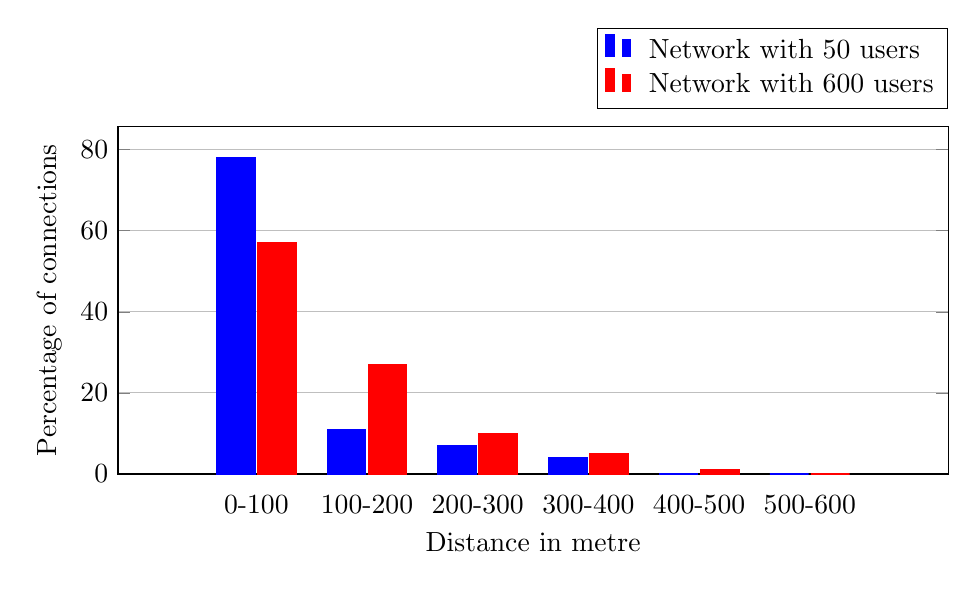
\begin{tikzpicture}
    \begin{axis}[
        width  = \textwidth,
        height = 6cm,
        major x tick style = transparent,
        ybar=2*\pgflinewidth,
        bar width=14pt,
        ymajorgrids = true,
        ylabel = {Percentage of connections},
        xlabel = {Distance in metre},
        symbolic x coords={0-100,100-200,200-300,300-400,400-500, 500-600},
        xtick = data,
        scaled y ticks = false,
        enlarge x limits=0.25,
        ymin=0,
        legend cell align=left,
        legend style={
                at={(1,1.05)},
                anchor=south east,
                column sep=1ex
        }
    ]
        \addplot[style={blue,fill=blue,mark=none}]
            coordinates {(0-100, 78) (100-200,11) (200-300,7) (300-400,4) (400-500,0) (500-600,0)};

        \addplot[style={red,fill=red,mark=none}]
            coordinates {(0-100, 57) (100-200,27) (200-300,10) (300-400,5) (400-500,1) (500-600,0)};

        \legend{Network with 50 users, Network with 600 users}
    \end{axis}

\end{tikzpicture}

      \caption{Distribution of how many connections belong to a certain interval of distance. Upper boundaries are not included.}
  \label{chart:distances}
\end{figure}

\section{Summary}
This chapter discussed the different formulas that will be used by the tool and how to program or optimize
some of the more complex problems like radiation patterns or path loss calculations.

First, the formulas about calculating the electromagnetic exposure from different sources and how they 
can be converted in \gls{SAR}-values are presented. The electromagnetic field radiation in the far-field 
and near-field can be converted with the constants $0.0028 \frac{W/kg}{W/m^2}$ and  $0.0070 \frac{W/kg}{W}$, respectively.
Secondly, a proper microstrip patch antenna 
has been defined, optimized for the 2.6 GHz frequency band.
The dimensions of the groundplane and glass substrate resulted in 52.4 mm by 43.8 mm and a height of 2.87 mm. The radiating patch 
itself has a width of 35.09 mm and a length of 26.55 mm.
Thereafter, the radiation pattern of this
antenna is achieved with the use of Matlab. 
Thirdly, a fitness function for the optimization strategy is introduced, explaining how this function will be able 
to optimize the network towards either electromagnetic exposure or network power consumption.
Eventually, the implementation itself is tackled  by discussing the main algorithm of the deployment tool and its embedded optimization 
algorithm. This is followed by an explanation on how a program can provide support 
for any possible radiation pattern.  Finally, some improvements towards the general performance are discussed
in order to reduce time complexity. The path loss calculations can be multithreaded, a proper data structure for neighbourhood search 
is introduced and non-essential computations are avoided by limiting the neighbourhood search to half a kilometre.

Once all these values and formulas have been implemented, the tool is ready to by applied to different scenarios which will 
be discussed in chapter \ref{chap:scenarios}.